\documentclass{article}
\usepackage[utf8]{inputenc}
\usepackage{graphicx}
\usepackage{float}
\usepackage{hyperref}

\title{ControlLab1}
\author{Nicholas Shindler}
\date{November 2019}

\begin{document}

\maketitle

\begin{center}
    email: \email{shindler25@gmail.com}\\
    code: \url{https://github.com/NickMcSweeney/ControlLab1}
\end{center}

\section{Question 1}
\subsection{Interface}
The "PID CONTROLLER" control unit box implemented for the Water Tank system is composed of 

\begin{itemize}
    \item A controller signal that governs automatic or manual input.
    \item F dial is the P value of a PID control.
    \item I is the I value of a PID control.
    \item D is the D value of a PID control.
    \item An Ext Set Value switch switches between a set value of 0 and the value set by the set value dial.
\end{itemize}




\subsection{Empirical tests}
We tested a set value of 3 (30\%) and achieved a good calibration result by setting $P=5$, $I=20$, $D=0.3$. This resulted in no overshoot and low oscillation at nearly the 30\% value.

\begin{figure}[H]
    \centering
    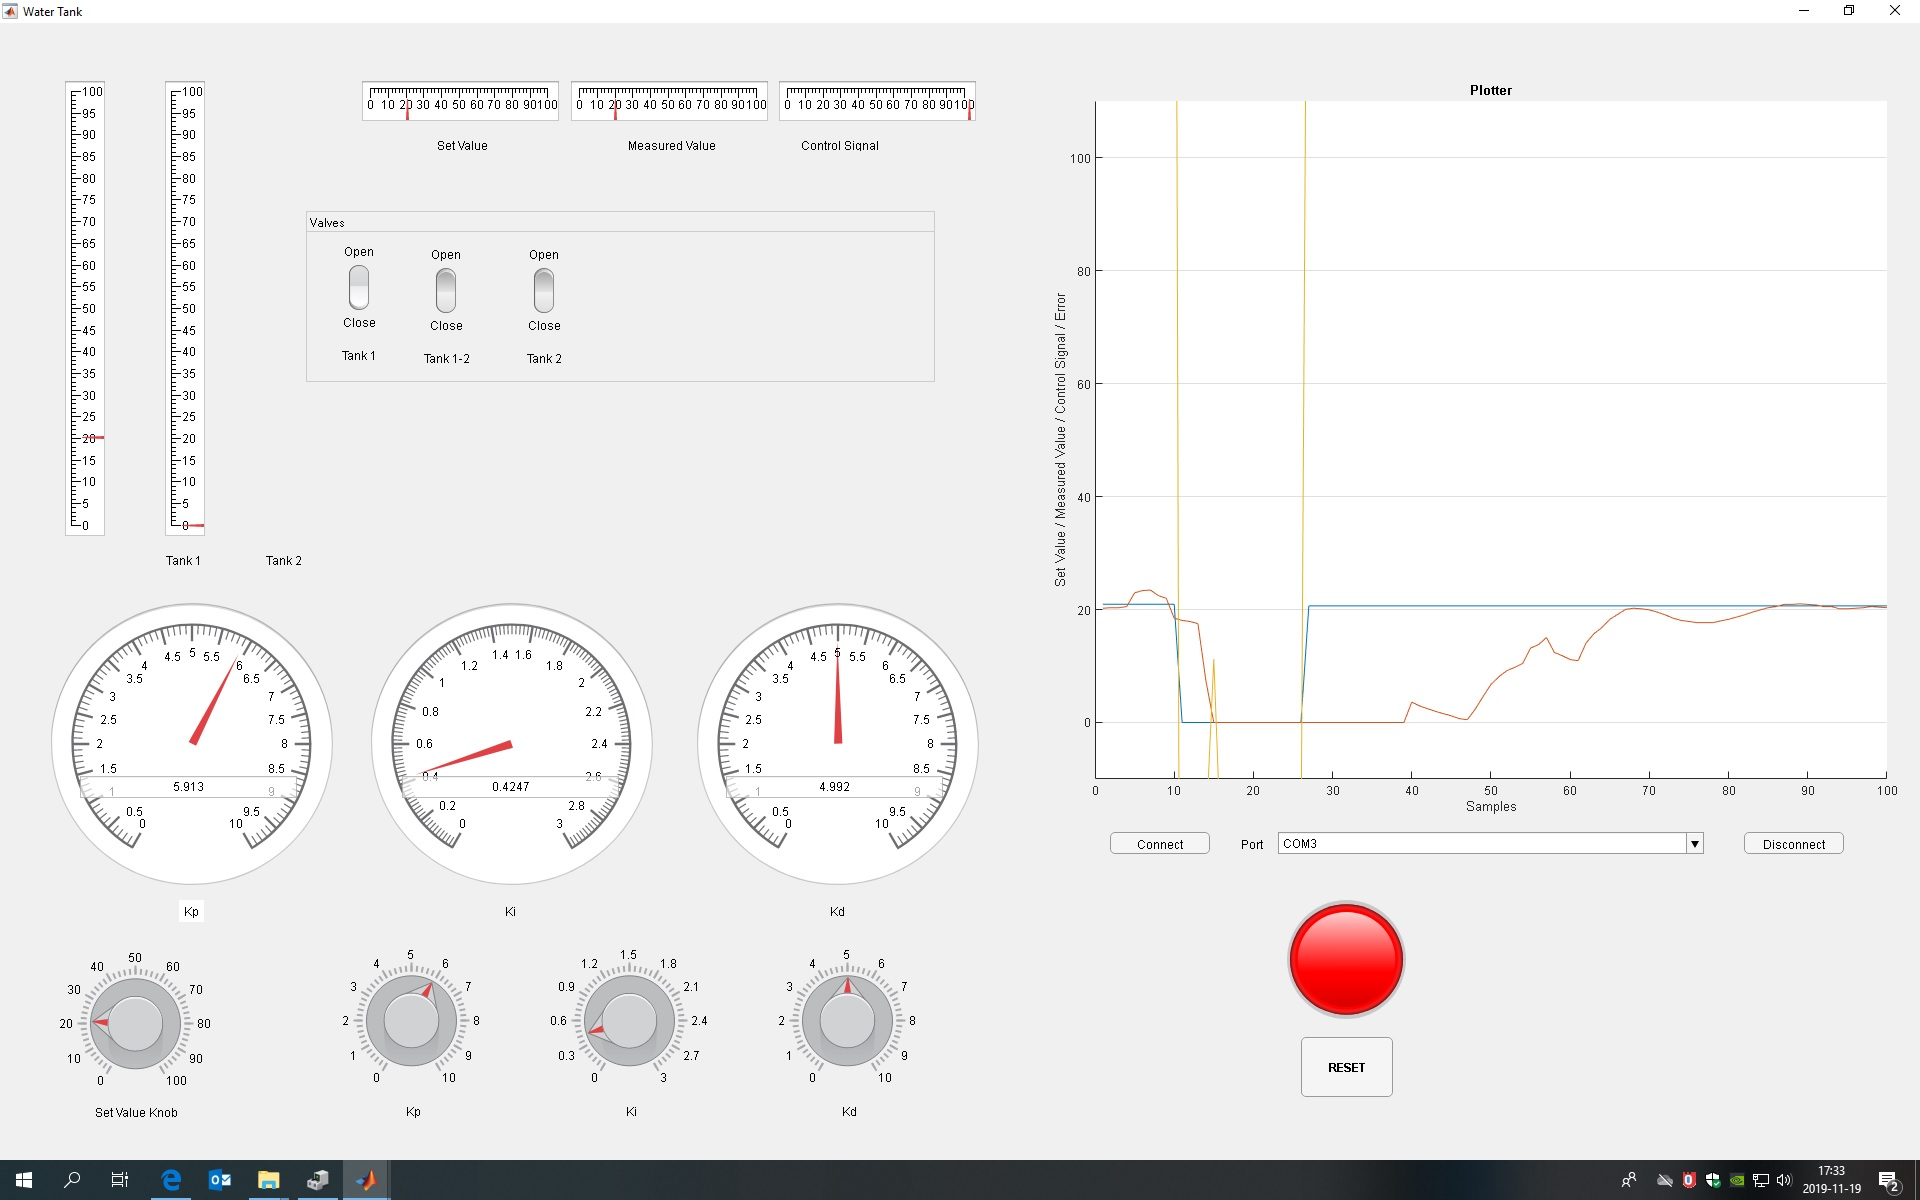
\includegraphics[width=0.6\textwidth]{PID_tune}
    \caption{PID tuning}
    \label{fig:PID_tune}
\end{figure}

\section{Question 2}
Given the parallel form of the equation:
\begin{equation} u(t) = K_p(e(t)) + K_i(\int_0^t e(t)dt) + K_d\frac{de(t)}{dt} \end{equation}
this board uses the standard equation
\begin{equation} u(t) = K_F((e(t)) + \frac{1}{K_I}(\int_0^t e(t)dt) + K_D\frac{de(t)}{dt}) \end{equation}

\section{Question 3}
\subsection{Initial regulator}
This is a binary controller. If there is error the motor is turned on to a set value ($96$), otherwise it is turned off.
\subsection{Regulator improvements}
We added a variable base motor speed and then added the error value to that to make the motor speed relative to how close it is to the set value.
\begin{equation} u(t) = set\ value*scalar1 + error*scalar2 \end{equation}
This addresses 2 problems. First, there is drainage that is relative to the volume of water. This is compensated by the $set_value \times scalar1$. Second, to get the water level to the set point and to stop we multiplied a scalar with the error.
\subsection{PID equation}
Initial calibration: $k_p = 5;\ k_d = 3;\ k_i = 0.6$ 
We used used the empirical testing from $q1$ as the baseline for calibration. Then, we fine tuned to get an initial rise that was quick and smooth.
End calibration: $k_p=5.913;\ k_i=0.4247;\ k_d=4.992$
we tuned at a value of 20 percent.

\section{Question 4}
\subsection{Tank simulator}
We implemented a model of the system in 2 different ways. We built a Simulink model implementing a built-in integrator and PID control functions. Using the PID control from the previous section, we tuned the $a,\ A,\ and\ \gamma$ values. 
\begin{figure}[H]
    \centering
    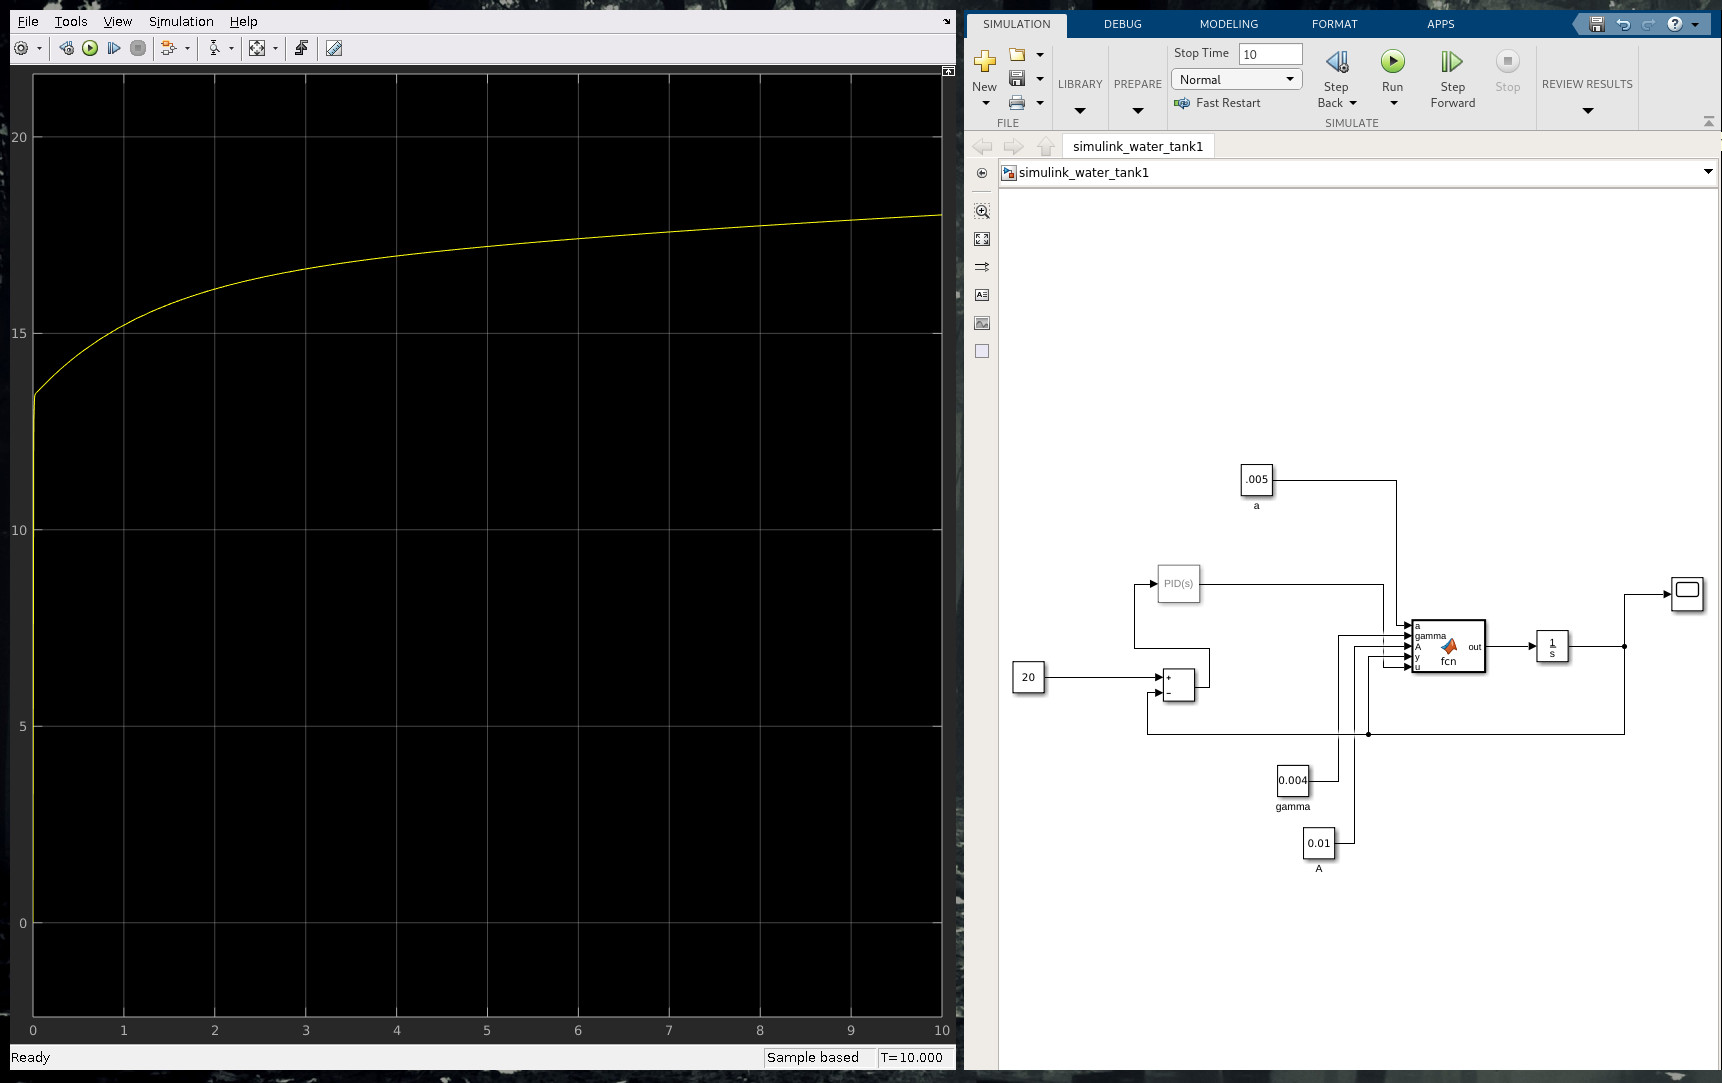
\includegraphics[width=0.8\textwidth]{simulink_model.jpg}
    \caption{Modeling the water tank system using Simulink}
    \label{fig:simulink}
\end{figure}

We additionally built a class to model the system and take inputs from the PID controller that we created, as well as using our own RK4 integrator function.
This resulted in values of $a=0.0021,\ A=0.008,\ and\ \gamma=0.001$. We determined these values through comparison of the water gain curves with the empirical tests, getting values such that our model performed like the real world tank for the set point we were using ($20$).

\end{document}

